\section{Ejercicio 3}
    % 1. Describir detalladamente el problema a resolver dando ejemplos del mismo y sus soluciones.
    \subsection{Descripción del problema}

        Gokú se está enfrentando a $N$ androides y necesita destruirlos con la menor cantidad de kamehamehas posibles. Los enemigos de Gokú se encuentran en posiciones $(X_i , Y_i)$ y los kamehamehas recorren una semirrecta desde donde Gokú lo lance, en cualquier dirección que Gokú lo decida, destruyendo a todos los androides que encuentren a su paso.

        Se desea escribir un algoritmo que tome la cantidad de androides $N$ y sus posiciones, y decida cuántos kamehameha debe lanzar Gokú y a qué enemigos destruye con cada uno de ellos. Si hay más de una solución óptima, se puede devolver cualquiera de ellas. Se debe utilizar la técnica de \emph{backtracking}, elaborando podas y estrategias para mejorar los tiempos de ejecución, y lograr una complejidad temporal $\ord(N^{N+2})$ o mejor.

        La salida que del algoritmo debe comenzar con la cantidad de kamehamehas usados. A continuación se debe agregar una línea por cada kamehameha, que debe contener la cantidad de androides destruidos por el mismo, seguido por los índices de dichos androides.

        Por ejemplo, para la siguiente entrada:
        
        \begin{verbatim}
        5
        0 0
        0 1
        0 2
        1 2
        2 2
        \end{verbatim}

        Una posible salida válida sería:

        \begin{verbatim}
        2
        3 3 4 5
        2 1 2
        \end{verbatim}

        Observación: Los kamehamehas matan a los androides. Esto significa que si un androide esta muerto, por mas que un kamehameha vuelva a pasar por encima de él, no vuelve a morir. Es por eso que:

        \begin{verbatim}
        2
        3 3 4 5
        3 1 2 3
        \end{verbatim}

        no es una salida válida, ya que estaría matando por segunda vez al androide ubicado en la posicion (0,2).
        
    % 2. Explicar de forma clara, sencilla, estructurada y concisa, las ideas desarrolladas para la resolución del problema. Utilizar pseudocódigo y lenguaje coloquial (no código fuente). Justificar por qué el procedimiento resuelve efectivamente el problema.
    \subsection{Solución propuesta}

    Como toda solución planteada siguiendo la técnica de \emph{bracktracking}, la solución se basa en probar todas las combinaciones posibles de kamehamehas, guardando para cada una de ellas la manera en que los androides son destruidos, para luego retornar la lista correspondiende a una de las soluciones que utilice una cantidad de kamehamehas óptima. Esto se hace de manera recursiva, llamando a una función que se encarga de probar cada kamehameha posible y para cada uno ramificarse, buscando destruir a los que hayan sobrevivido.

    Teniendo en cuenta que cualquier par de androides puede ser eliminado con un único kamehameha, en ningún caso (suponiendo $N \geq 2$) será conveniente realizar un disparo que no aniquile al menos a dos enemigos. Por lo tanto, se considerará que los kamehamehas que se pueden disparar están dados por los todos los pares de androides posibles. Lanzar un kamehameha consiste en tomar la recta que pasa por estos dos androides, y luego, recorrer todos los demás enemigos, determinando cuáles de ellos son destruidos por ese disparo. A continuación, se utiliza la recursión para encontrar la forma óptima de matar a los androides restantes.

    Los casos base de la recursión son triviales, y están planteados para $N = 0$ (no se realiza ningún disparo) y $N =1$ o $N = 2$ (se dispara un único kamehameha que mata a todos los androides). En los demás casos, por la naturaleza de la recursión, para cada posibilidad para el primer disparo se habrá obtenido la solución óptima para destruir a los enemigos restantes; por lo tanto basta con elegir, de entre estas opciones, aquella cuya solución recursiva utilice la cantidad de disparos mínima.

    Si se analiza la forma en que se construye la solución, resulta claro que la respuesta del algoritmo planteado es efectivamente una solución correcta del problema. Por un lado, todos los enemigos son necesariamente destruidos en algún nivel de la recursión. Además, dado que al finalizar la ejecución se habrán recorrido todas las posibles combinaciones de disparos, es posible asegurar que se encontrará, efectivamente, aquella cuya cantidad de kamehamehas sea mínima. 

    \subsubsection{Podas y otras mejoras diseñadas}

    Desde luego, si bien se acaba de presentar una solución válida al problema, Gokú podría verse en apuros si debiera utilizarla para frenar una invasión inminente de androides, dado que el costo computacional de probar todos los kamehamehas posibles puede resultar excesivamente alto. Es por eso que se decidió implementar una serie de podas y otras metodologías que permitieran mejorar la eficiencia del algoritmo.

    \begin{enumerate}
        \item La primer estrategia que se incorporó consistió en evitar la repetición trivial de kamehamehas: resulta evidente que el kamehameha dado por el par de androides $(a_1, a_2)$ es el mismo que el dado por $(a_2, a_1)$. Por esta razón, se modificó la metodología utilizada para recorrer los enemigos, implementando dos ciclos, en donde el exterior (correspondiente a $a_1$) recorre todos los androides, y el interior (correspondiente a $a_2$) solo recorre los androides de $a_1$ en adelante.

        \begin{codesnippet}
        \begin{verbatim}
            para i entre 0 y cantidadDeAndroides - 1 hacer:
             |  para j entre i y cantidadDeAndroides - 1 hacer:
             |   |  lanzarKamehameha(i, j)
             |  fin para
            fin para
        \end{verbatim}
        \end{codesnippet}

        Dado que tras esta modificación aún se siguen intentado todos los disparos posibles, resulta claro que al agregarla no se altera la correctitud del algoritmo.

        \item Si bien ya no se repiten pares de androides, aún puede existir algunos kamehamehas superpuestos; este es el caso en el que se selecciona un par de andorides y aparece un tercero en la misma recta. Por ejemplo, el kamehameha que pasa por (0,0) y (1,1) es el mismo que pasa por (1,1) y (2,2). Estos kamehamehas redundantes también pueden omitirse, evitando llamadas recursivas innecesarias sin afectar en absoluto el resultado del algoritmo.

        Para implementar esta estrategia, se decidió ir almacenando los disparos efectuados. Luego, al seleccionar un par de androides distintos, antes de realizar la llamada recursiva correspondiente, se verifica que el disparo no resulte redundante con uno que ya se haya realizado con anterioridad durante la misma rama de ejecución (podría usarse ese mismo kamehameha, pero en una rama diferente).

        \item La última poda diseñada se basa en la idea de que, en muchos casos, es posible determinar que una rama de la recursión no producirá una solución óptima sin necesidad de ejecutarla hasta el final. Esto puede hacerse almacenando la cantidad de kamehamehas usados por la mejor solución hallada hasta el momento, y pasando dicho valor por parámetro en cada llamada recursiva. Dicho valor funciona como un ``tope'' para la profundidad de la recursión: dado que cada nivel recursivo agrega un kamehameha a la solución, cuando una determinada rama de ejecución alcanza dicho tope de profundidad sin haber llegado a una solución válida, esto significa que la mencionada rama no podrá aportar una solución mejor que una que ya se obtuvo con anterioridad y, por lo tanto, puede descartarse sin problemas. En este caso se detiene la ejecución de la rama y se comunica al nivel superior de la recursión que no se obtuvo un resultado válido.

        Es importante señalar que ninguna rama se descarta a menos que se tenga la seguridad de que no producirá un resultado correcto. Por lo tanto, nuevamente, la correctitud del algoritmo no se ve afectada.

    \end{enumerate}

    \subsubsection{Detalles implementativos}
    
    El algoritmo fue implementado en lenguaje C++. Para almacenar la solución, se recurre a la clase \texttt{vector}, proporcionada por la librería estándar del lenguaje.

    Durante la ejecución del algoritmo se utilizan dos variables globales; un entero para almacenar la cantidad de enemigos y un vector que contiene la ubicación de cada uno de ellos. La ejecución consiste principalmente de una función recursiva, que presenta las siguientes características:

    \begin{itemize}
        \item Se prueban todos los pares de enemigos posibles mediante dos ciclos anidados, de la forma que se describe en el primer punto de la sección anterior.
        \item Dentro del ciclo interior se revisa a qué enemigos destruye el kamehameha descripto por el par de enemigos elegido y se destruyen esos enemigos para luego agregarlos a la solución.
        \item Destruir los enemigos consiste en eliminarlos de un vector que contiene a los enemigos restantes. Este vector es una copia del vector de enemigos restantes; el original debe conservarse porque, para cada kamehameha distinto, el algoritmo se bifurca con diferentes enemigos restantes.
        \item Agregarlos a la solución consiste en añadir un vector que contiene a dichos enemigos a un vector de vectores, que representa la solución parcial construida hasta el momento: cada posición del vector corresponde a un kamehameha distinto y contiene a los enemigos que el mismo destruye.
        \item Sus casos base son las llamadas donde la cantidad de enemigos restantes es igual o menor que 2. Estos casos no necesitan realizar llamadas recursivas, y simplemente devuelven un vector cuyo único enemigo es el vector de los enemigos a destruir, ya que estos pueden ser liquidados con un único kamehameha.
    \end{itemize}

    % hecho. Deducir una cota de complejidad temporal del algoritmo propuesto y justificar por qué el algoritmo cumple la cota dada. Utilizar el modelo uniforme.
    \subsection{Complejidad teórica}

    Al comienzo se inicializa un vector de $N$ posiciones, lo cual tiene costo del orden de $N$. El algoritmo consiste principalmente de una función recursiva, cuyo costo determina la complejidad temporal total de la solución.
    
    Dicha función contiene dos ciclos, un dentro del otro; el ciclo exterior recorre índices desde $0$ hasta $N - 1$, y el interior, desde $i$ hasta $N$. Esto implica que lo implementado dentro del ciclo interior se ejecute $N \times (N - 1)$ veces. Analizando este último ciclo, puede verse que:

    \begin{itemize}
        \item Se recorren todos los kamehamehas anteriormente lanzados, que a lo sumo pueden ser $N/2$, ya que cada kamehameha elimina al menos a 2 androides. Esto tiene un costo del orden de $N$.
        \item Se destruyen los enemigos alcanzados por el kamehameha. Esto consiste en recorrerlos todos (ciclo con orden de $N$ iteraciones) y borrar cada uno del vector donde estan almacenados (esto cuesta también $\ord(N)$), con un costo del orden de $N^2$. Luego se los agrega a un vector con enemigos destruidos, con un costo del orden de $N$. Por lo tanto, el costo total es del orden de $N^2$.
        \item Por último se llama a la misma función en forma recursiva.
    \end{itemize}

    Se debe observar que al hacer el nuevo llamado, la cantidad de enemigos va a haber disminuido al menos en 2. Debido a esto, dentro de la siguiente llamada, el ciclo exterior recorrerá solo $N - 2$ indices y el interior $N - 3$. Así estas cantidades disminuirán de a 2 hasta terminar, llegando a 1.

    %% IMPORTANTE: LLEGUÉ A REVISAR HASTA ACÁ.

    Si pensamos la cantidad de llamadas recursivas como un árbol donde cada node es una llamada, tenemos un árbol de a lo sumo $N/2$ niveles, donde en su primer nivel hay $N \times (N - 1)$ llamados. Cada uno tiene $(N - 2) \times (N - 3)$ hijos, a su vez cada uno de ellos $(N - 4) \times (N - 5)$ y así sucesivamente hasta llegar a 1. Por lo que en el segundo nivel habrán $N \times (N - 1) \times (N - 2) \times (N - 3)$ nodos, y de esta forma en el último nivel se encontraran $N!$ hojas.

    El árbol no puede tener más de $N/2$ niveles ya que cada nivel representa un kamehameha, y no pueden haber más de $N/2$ kamehamehas.

    Ejemplo para $N$ = 4: 

    \begin{center}
    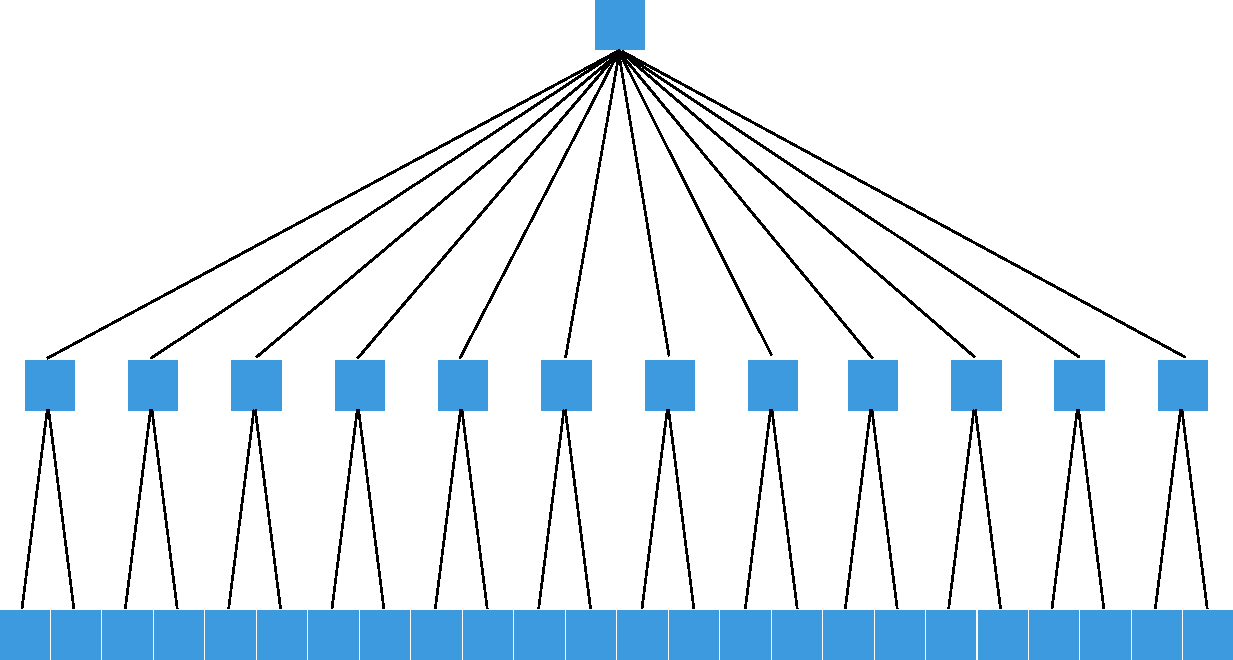
\includegraphics[width=0.6\columnwidth]{imagenes/ej3_arbol.pdf}
    \end{center}
    
    Se puede ver como para el caso de $N = 4$ tenemos que la raiz tiene $4 \times 3 = 12$ hijos y que cada uno tiene $2 \times 1 = 2$ hijos. En otras palabras, en la primera ejecución (la raíz) se hacen 12 llamados (uno por cada par de enemigos), y para cada uno se hacen dos llamados (uno por cada par de enemigos restantes).

    En el nivel $k$ con $0 \leq k \leq N / 2$ se puede ver que cada nodo tiene $(N - 2k) \times (N - 2k - 1)$ hijos,
    debido a los ciclos explicados previamente. Entonces la cantidad de nodos en el nivel $k$ está dada por la cantidad de nodos en $k - 1$ multiplcado por $(N - 2k) \times (N - 2k -1)$. De esta forma la cantidad de nodos en el nivel $k$ es igual al producto de las cantidades de hijos por nodo de cada nivel, hasta $k$. Es decir, 

    \[\text{\#nodos en nivel }k = \prod_{l = 0}^{k}(N - 2l) \times (N - 2l -1)\]

    Y por lo tanto se cumple para el último nivel ($k = N/2$) donde los nodos son hojas

    \[\text{\#hojas }= \prod_{l = 0}^{N / 2}(N - 2l) \times (N - 2l -1) = N!\]

    Sabiendo que la cantidad de hojas es $N!$ y la altura es $N/2$, y que cada llamada tiene un costo de orden $N^2$, se puede pensar que este arbol de ejecución está acotado superiormente por una ``matriz'' de $N/2$ filas y $N!$ columnas donde cada elemento es una llamada de costo $N^2$.

    Es decir, la complejidad del algoritmo está acotada superiormente por $N/2 \times N! \times N^2$ que es de orden $N^3 \times N!$.

    Ahora veremos que vale $N^k \times N! \leq k! \times N^N$ $\forall k$ constante, particularmente lo vale para $k = 3$, y que por lo tanto $N^3 \times N!$ está acotado superiormente por $N^N$ que a su vez está acotado por $N^{N + 2}$, por lo que el algortimo cumple la complejidad requerida.

    \[ N^N = \prod_{i = 0}^{n - 1}n = N^k \times \prod_{i = 0}^{N - k - 1} N \geq N^k \times \prod_{i = 0}^{N - k - 1} (N - 1) = N^k \times \frac{N!}{k!}\]

    Dado que $N^N \geq N^k \times \frac{N!}{k!} \implies k! \times N^N \geq N^k \times N!$ y por lo tanto $N^k \times N! \in \ord(N^N) \forall k \in \nat$

    % 4. Dar un código fuente claro que implemente la solución propuesta. Se deben incluir las partes relevantes del código como apéndice del informe impreso entregado.

    % 5. Realizar una experimentación computacional para medir la performance del programa implementado. Usar un conjunto de casos de test en función de los parámetros de entrada, con instancias aleatorias e instancias particulares (de peor/mejor caso en tiempo de ejecución, por ejemplo). Presentar en forma gráfica una comparación entre los tiempos medidos y la complejidad teórica calculada y extraer conclusiones.
    \subsection{Experimentación}

        Al igual que con los otros dos ejercicios, se realizaron pruebas experimentales para verificar que el tiempo de ejecución del algoritmo cumpliera con la cota asintótica de $\ord(N^{N+2})$, teóricamente demostrada para el peor caso. Se realizaron dos tipos de pruebas:
        
        \begin{itemize}
            \item Pruebas con instancias con características particulares, más específicamente, para el mejor caso, el peor caso y casos intermedios.
            \item Pruebas con instancias generadas aleatoriamente, para obtener una aproximación al comportamiento del algoritmo en el caso promedio.
        \end{itemize}

        \subsubsection{Instancias particulares}

            Todas las instancias utilizadas para estas pruebas se generaron de manera aleatoria, pero restringiendo los resultados obtenidos para cumplir con determinadas características. A continuación se enumeran los criterios tenidos en cuenta para la generación de los escenarios de prueba.

            \begin{itemize}
                \item \textbf{Mejor caso:} El mejor caso del algoritmo se produce cuando todos los androides a destruir están ubicados sobre una única línea recta. En este caso, es seguro que el primer kamehameha con el que se intente será la solución óptima del problema, por lo que solo se bajará por esa rama de la recursión.

                \item \textbf{Peor caso:} El peor caso del algoritmo se da cuando no existen tres androides alineados a destruir. En consecuencia, cada kamehameha destruirá tan solo dos enemigos, que es el mínimo posible. Esto maximiza la complejidad temporal del algoritmo por dos motivos. Por un lado, en cada nivel de la recursión, se intentarán disparar todos los kamehamehas posibles, con la esperanza de que pueda encontrarse una solución más razonable. Por otra parte, en cada llamada recursiva que se efectúe, la entrada solo se reducirá en dos elementos, haciendo que la profundidad de la recursión alcance siempre la cota máxima de $\frac{N}{2}$.

                \item \textbf{Caso intermedio:} También se agregó un escenario de prueba adicional, con el objetivo principal de poner a prueba la efectividad de las podas implementadas. El mismo consiste en la combinación de dos instancias de mejor caso de tamaño $\frac{N}{2}$; es decir, la mitad de los androides se encuentran sobre una línea recta y la otra mitad, sobre una recta diferente. Las coordenadas de los enemigos son mezcladas de forma aleatoria para evitar que el kamehameha óptimo sea necesariamente el primero que se intente.
                
                Bajo estas condiciones, cabe esperar que las podas entren en acción, reduciendo considerablemente cantidad de llamadas recursivas que se ejecutan completas y consiguiendo un rendimiento apreciablemente superior al observado en el peor caso.

                Cabe destacar que este es un simple caso adicional de prueba, concebido con el objetivo de ilustrar la gran variación en el rendimiento del algoritmo según las características de los datos de entrada, pero que no guarda relación alguna con el comportamiento del algoritmo en el caso promedio.
            \end{itemize}

            Para los tres escenarios previstos, se generaron instancias de prueba para todos los valores de $N$ entre $1$ y $12$, inclusive. Luego, en cada caso, se ejecutaron $60$ repeticiones del algoritmo, midiendo cada vez el tiempo de ejecución y tomando luego el promedio entre los resultados obtenidos.

            En un principio, se descubrió que se producían picos en el tiempo de ejecución en las primeras corridas del programa, tendiendo los valores a estabilizarse con las sucesivas corridas. Si bien no se pudo determinar con precisión el origen de estas anomalías, se decidió, para minimizar la varianza de los datos obtenidos, tratar a las primeras $20$ repeticiones de cada instancia como \emph{outliers}, y promediar solo los valores de las últimas $40$.

            \renewcommand\constante{0.001}

            Los resultados obtenidos se exponen en el gráfico de la Figura \ref{fig:exp3:part_tiempo_base}, donde se ilustra también la cota teórica de $c \times N^{N + 2}$ (el valor de $c$ utilizado es \constante). Se representan como $T_P$ los tiempos obtenidos para peor caso, como $T_M$ para el mejor caso, y como $T_I$ para el caso intermedio. Puede observarse claramente que, incluso en el peor escenario, el tiempo de ejecución del algoritmo tiende a aumentar a un ritmo estrictamente más lento que el de la cota prevista.

            \begin{figure}[H]
                \centering
                \caption{}
                \label{fig:exp3:part_tiempo_base}
                \begin{tikzpicture}
                    \begin{axis}[
                            title={},
                            xlabel={Tamaño de entrada ($N$)},
                            ylabel={Tiempo de ejecución (nanosegundos)},
                            ymode = log,
                            scaled x ticks=false,
                            scaled y ticks=false,
                            enlargelimits=0.05,
                            width=0.5\textwidth,
                            height=0.5\textwidth,
                            legend pos=north west,
                            legend cell align=left,
                            xmin=1
                        ]

                        \addplot[color=red] table[x index=0,y index=1]{../exp/kamehamehaPeor};
                        \addplot[color=blue] table[x index=0,y index=1]{../exp/kamehamehaIntermedio};
                        \addplot[color=green] table[x index=0,y index=1]{../exp/kamehamehaMejor};
                        \addplot[color=gray] table[x index=0, y expr={\constante * (x^(x+2))}]{../exp/kamehamehaPeor};
                        \legend{$T_P(N)$, $T_M(N)$, $T_I(N)$, $c \times N^{N+2}$}
                    \end{axis}
                \end{tikzpicture}
            \end{figure}

            En la Figura \ref{fig:exp3:part_tiempo_sobre_exp} se muestra el cociente entre los datos obtenidos y la función $\times N^{N + 2}$ (se considera el mismo valor de $c$ que en el gráfico anterior). Puede observarse como, al aumentar el tamaño de $N$, el cociente se aproxima rápidamente a $0$, ilustrando el hecho de que el crecimiento asintótico de la cota es estrictamente mayor que el de los tiempos obtenidos en las mediciones.

            \begin{figure}[H]
                \centering
                \caption{}
                \label{fig:exp3:part_tiempo_sobre_exp}
                \begin{tikzpicture}
                    \begin{axis}[
                            title={},
                            xlabel={Tamaño de entrada ($N$)},
                            ylabel={Tiempo de ejecución (nanosegundos)},
                            ymode = log,
                            scaled x ticks=false,
                            scaled y ticks=false,
                            enlargelimits=0.05,
                            width=0.5\textwidth,
                            height=0.5\textwidth,
                            legend pos=north west,
                            legend cell align=left,
                            xmin=1
                        ]

                        \addplot[color=red] table[x index=0,y expr={\thisrowno{1} / (x^(x+2))}]{../exp/kamehamehaPeor};
                        \addplot[color=blue] table[x index=0,y expr={\thisrowno{1} / (x^(x+2))}]{../exp/kamehamehaIntermedio};
                        \addplot[color=green] table[x index=0,y expr={\thisrowno{1} / (x^(x+2))}]{../exp/kamehamehaMejor};
                        \addplot[color=gray] table[x index=0, y expr={\constante}]{../exp/kamehamehaPeor};
                        \legend{$\frac{T_P(N)}{N^{N+2}}$, $\frac{T_M(N)}{N^{N+2}}$, $\frac{T_I(N)}{N^{N+2}}$, $c$}
                    \end{axis}
                \end{tikzpicture}
            \end{figure}

            El análisis expuesto de los datos recopilados presenta evidencia empírica sobre la pertinencia la cota de complejidad demostrada teóricamente. Más aún, permite llegar a la conclusión que, incluso en las instancias de peor caso, esta cota resulta holgada, es decir, que la complejidad del algoritmo presentado es estrictamente $\ord(N^{N+2})$.

        \subsubsection{Instancias aleatorias}

            Para obtener una aproximación al comportamiento del algoritmo en el caso promedio, se realizaron también pruebas con instancias generadas de forma completamente aleatoria. Este experimento también se realizó para los valores de $N$ entre $1$ y $12$, y al igual que el anterior, la prueba se repitió $60$ veces para cada valor de $N$, descartando los resultados de las primeras $20$ repeticiones y promediando los obtenidos en las otras $40$. Sin embargo, esta vez cada medición se realizó sobre una instancia de prueba diferente, generada al azar.

            Intuitivamente, resulta razonable conjeturar que la probabilidad de que al tres enemigos se encuentren alineados en una instancia aleatoria es muy baja, especialmente teniendo en cuenta los pequeños tamaños de entrada considerados. En otras palabras, parece esperable que un escenario aleatorio tenga características similares a un escenario de peor caso, y por lo tanto, que el rendimiento promedio del algoritmo sea similar a este último caso.

            En la figura \ref{fig:exp3:random_tiempo} se presentan los resultados obtenidos para estas instancias aleatorias ($T_R$), y se los compara con los previamente obtenidos para las instancias de peor caso ($T_P$). Como puede observarse, los datos empíricos respaldan la hipótesis recién expuesta. Cabe destacar que, a pesar de que todas las mediciones se realizaron sobre instancias diferentes, la varianza muestral observada fue comparable a la obtenida para el peor caso, donde las repeticiones se efectuaban con instancias idénticas, mostrando cierta uniformidad en el rendimiento del algoritmo cuando los datos de entrada no cumplen características particulares que permitan aprovechar las podas diseñadas.

            \begin{figure}[H]
                \centering
                \caption{}
                \label{fig:exp3:random_tiempo}
                \begin{tikzpicture}
                    \begin{axis}[
                            title={},
                            xlabel={Tamaño de entrada ($N$)},
                            ylabel={Tiempo de ejecución (nanosegundos)},
                            ymode = log,
                            scaled x ticks=false,
                            scaled y ticks=false,
                            enlargelimits=0.05,
                            width=0.5\textwidth,
                            height=0.5\textwidth,
                            legend pos=north west,
                            legend cell align=left,
                            xmin=1
                        ]
                        \addplot[color=red] table[x index=0, y index=1]{../exp/kamehamehaRandom};
                        \addplot[color=gray] table[x index=0, y index=1]{../exp/kamehamehaPeor};
                        \legend{$T_R(N)$, $T_P(N)$}
                    \end{axis}
                \end{tikzpicture}
            \end{figure}